\section{Persona} 

In diesem Abschnitt wird die im Zuge dieser Ausarbeitung entwickelte Persona vorgestellt.
Bei einer realen Umsetzung der NOG werden mehrerer Personas erstellt, damit ein möglichst breites Spektrum der Nutzenden in diesen abgebildet wird.
Die Persona dient im Folgenden auch als Handelnder im unter \autoref{sec:istSzenario} aufgeführten IST-Szenario.

\autoref{fig:personaPaul} zeigt eine grafische Beschreibung der Persona Paul Theiss, welche im Folgenden als fiktiver Repräsentant eines Steuerfahnders auftritt.
Paul ist 45 Jahre alt, verheiratet und hat zwei Kinder.
Er arbeitet seit Berufseintritt in der hessischen Finanzverwaltung.
In seiner Freizeit verbringt Paul gerne Zeit mit seiner Familie.
Wichtig anzumerken ist, dass Paul als fiktive Person die Entwicklung des momentan verwendeten Meldekopfsystems zugeschrieben wird. 
Weitere Informationen zur Persona Paul Theiss sind wie erwähnt \autoref{fig:personaPaul} zu entnehmen

Die im Folgenden zu findenden Handlungen und Personen sind erfunden. Ähnlichkeiten mit lebenden oder toten Personen sowie Handlungen sind rein zufällig. 

\begin{figure}
    \centering
    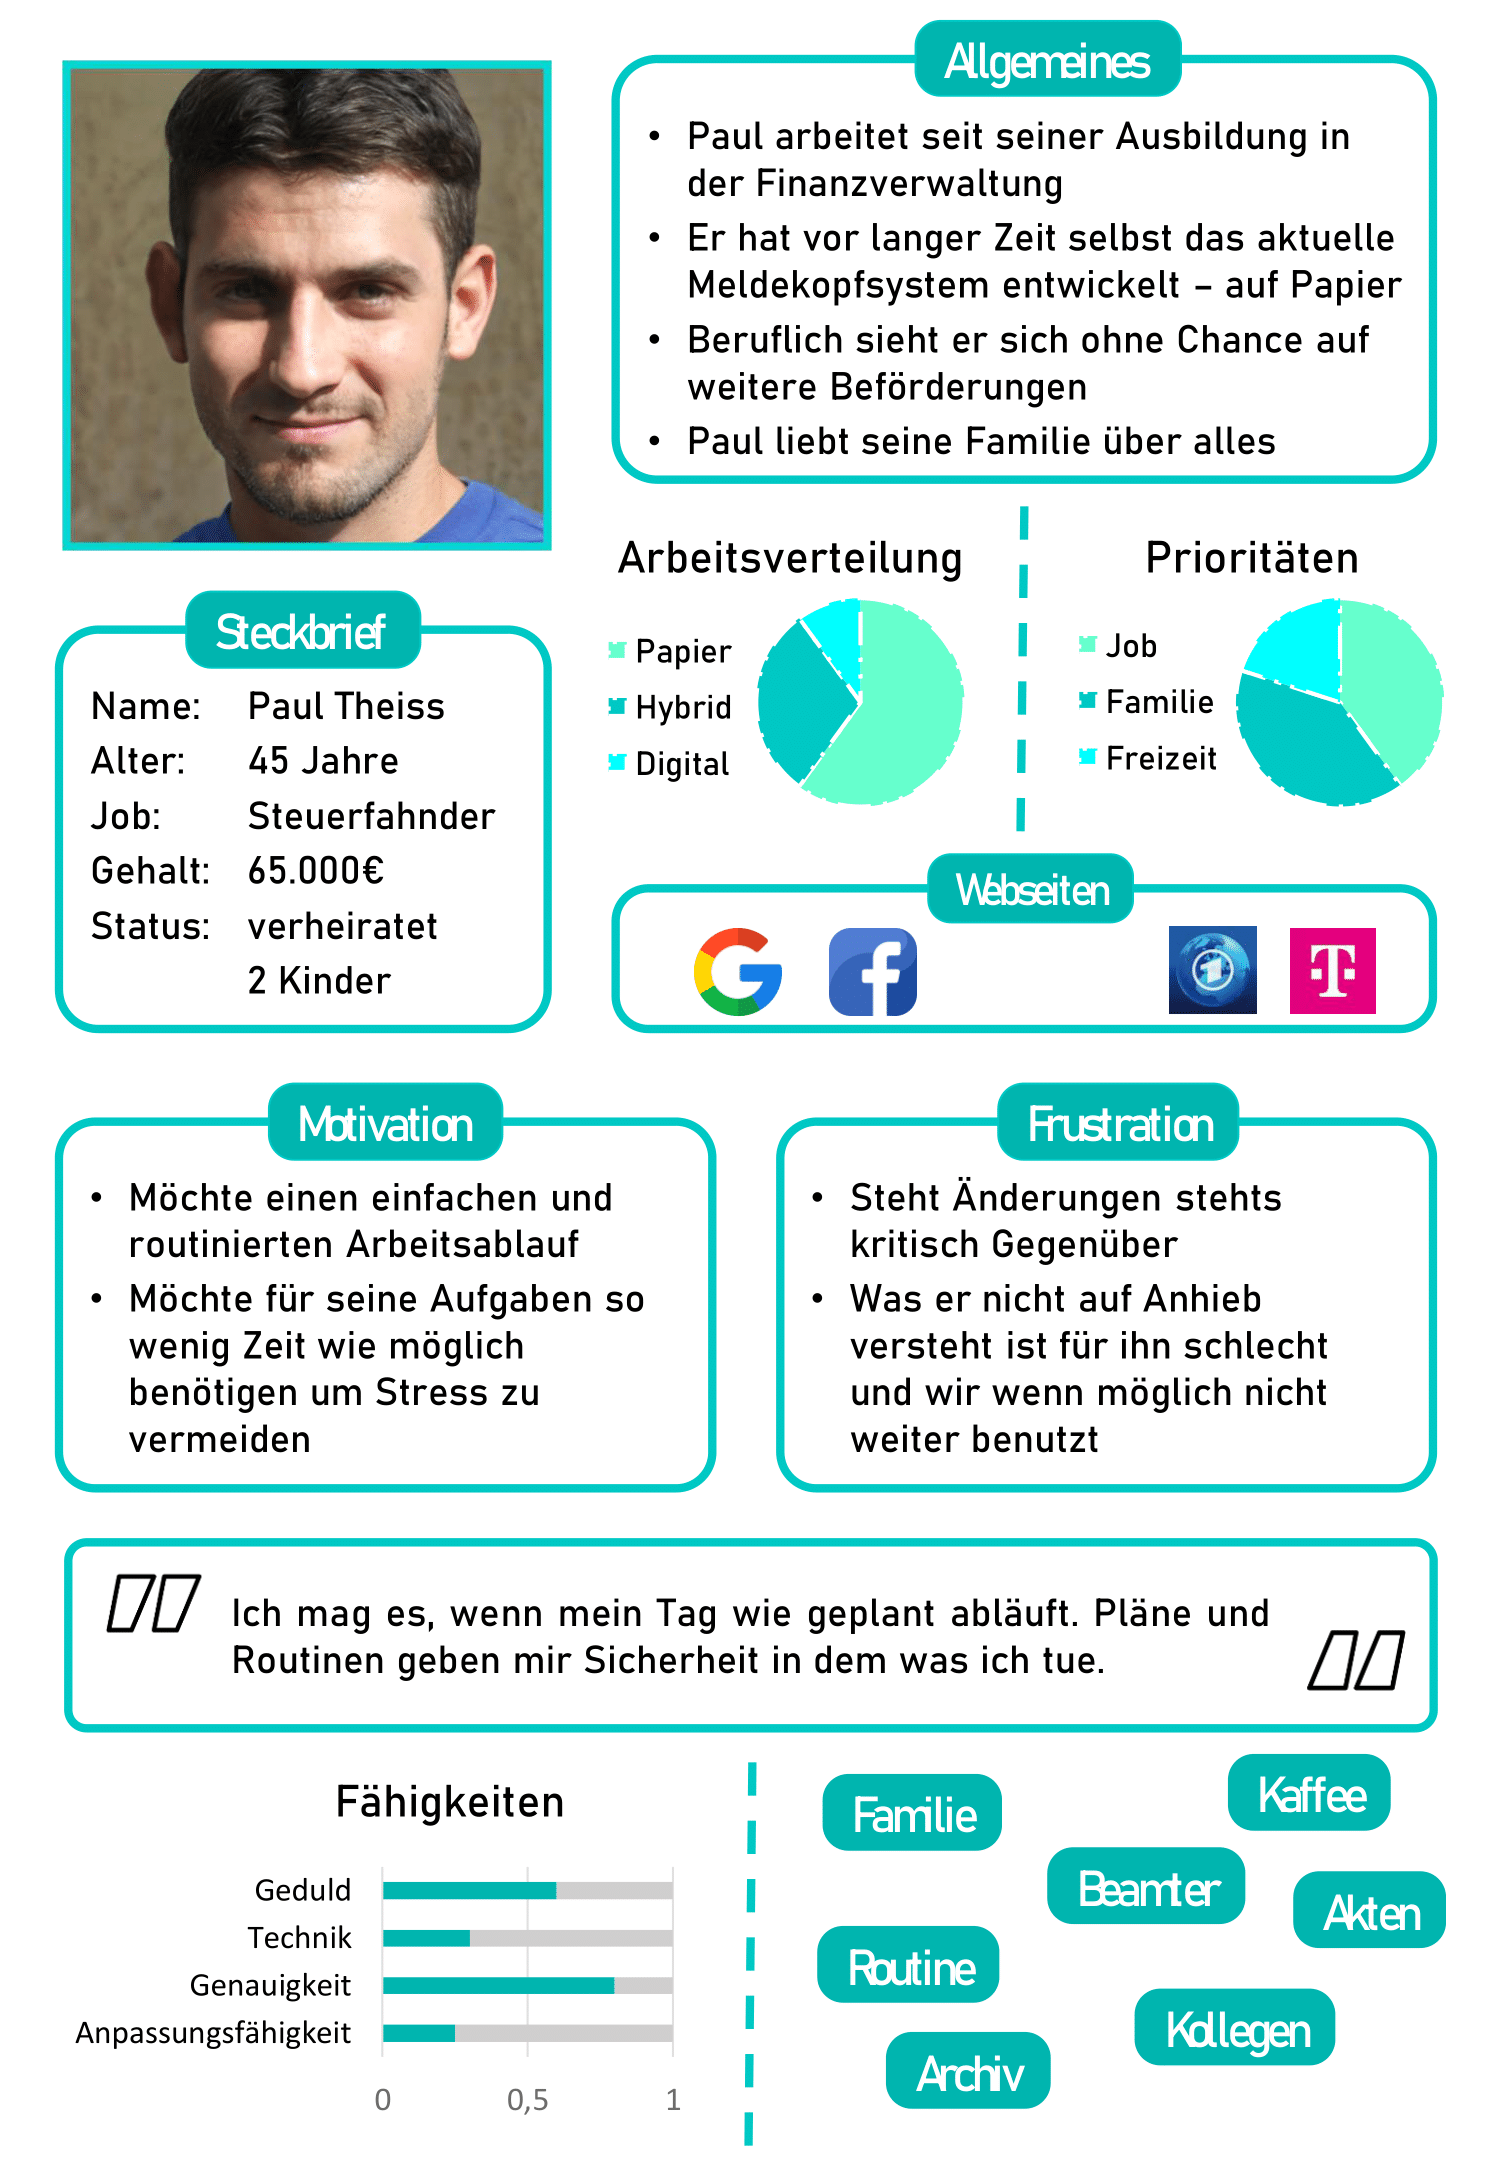
\includegraphics[width=\textwidth]{images/persona_1.png}
    \caption{Persona Paul Theiss}
    \label{fig:personaPaul}
\end{figure}